\documentclass[a4paper, 12pt]{abntex2}
\usepackage[utf8]{inputenc}
\usepackage{indentfirst}
\usepackage[space]{grffile}
\usepackage{graphicx}
\usepackage[margin=0.5in]{geometry}
\usepackage{float}
\usepackage{mathtools,mathrsfs}
%\usepackage[nottoc]{tocbibind} %make tableofcontents
\usepackage{titlesec}
\usepackage{subcaption}
\usepackage{xcolor,colortbl}
\usepackage{makecell}
\usepackage{cite}
\usepackage{bibentry}
\nobibliography*
\definecolor{gray}{rgb}{0.5,0.5,0.5}
\selectlanguage{brazil}
\makeindex

\instituicao{%
Universidade de São Paulo - Escola Politécnica
\par
Projeto de Pesquisa para Mestrado}

\titulo{Estudo de sinais mecânico-elétricos cardíacos}
\autor{Bernardo Mascarenhas Camargos e Silva}
\orientador{Sérgio Shiguemi Furuie}
\data{\today}
%Tira a pagina extra em branco
\openany
\begin{document}
% Retira espaço extra obsoleto entre as frases.
\frenchspacing
    \imprimirfolhaderosto

    \tableofcontents*
    \newpage
    
    \chapter{Introdução}

    Os métodos comumente utilizados de sensoriamento do coração podem ser separados em três classes, a detecção de sinais elétrico gerados pelo sistema cardíaco, geralmente feita por ECG, a detecção das movimentações mecânicas do sistema cardíaco, geralmente feita por fonocardiograma, e a observação do coração por métodos de visualização, geralmente feito por ecocardiograma. Embora a terceira classe tenha uma capacidade de diagnostico superior as outras ela exige um ambiente controlado e geralmente um maquinário grande e de alto custo, e portanto não será foco desse estudo.

    A detecção de sinais elétricos cardíacos por meio do eletrocardiograma (ECG)  é usualmente o método padrão de sensoriamento contínuo utilizado, uma vez que o sinal elétrico cardíaco tem relativamente pouca variação, mesmo comparando o sinal de diferentes pacientes, e já foi amplamente estudado, tornando sua análise simples e sua detecção bem padronizada e de fácil implementação, tornando detecção de eventos simples, como batimentos por minuto (bpm), fácil e confiável. O problema da detecção do sinal elétrico é que esse é o ativador das etapas do ciclo cardíaco, portanto não temos informação direta sobre o movimento real do coração, somente a influência que esse tem sobre o sinal elétrico seguinte.

    Por outro lado, a detecção dos sinais mecânicos do sistema cardíaco é realizada, quase exclusivamente, por fonocardiograma (PCG), que é a detecção do som produzido pelo ciclo cardíaco, e geralmente de forma não automatizada, ou seja é geralmente realizada pelo médico utilizando um estetoscópio e seu conhecimento para detectar e analisar o sinal. Essa técnica permite ao médico uma análise qualitativa do estado atual do coração do paciente, mas, por ser uma técnica dependente da audição do médico, não permite uma análise quantitativa, além de depender da capacidade do médico que esta realizando a técnica.%Preciso checar se isso é verdade e pegar umas fontes
Diversas tentativas de automatizar esse processo estão sendo feitas, mas ainda não estão sendo utilizadas na prática. %Preciso de referências e razão da dificuldade 

    Outros dois métodos de sensoriamento mecânico do ciclo cardíaco que estão ganhado espaço e atenção nas pesquisas teóricas da área são o balistocardiograma (BCG) e o seismeocaridograma (SCG). Esses dois métodos foram continuamente estudados durante o século 20, mas devido a problemas tecnológicos e ao avanço de outros tipos de medições foram deixados de lado, e somente agora estão ganhando novamente seu espaço entre os métodos de sensoriamento \cite{ballistoAndSeisReview}.
    
    O balistocardiograma tem como objetivo observar as vibrações no corpo geradas pela ejecção de sangue do sistema cardíaco, geralmente realizado por meio de uma balança, uma cadeira ou uma cama com sensoriamento. Como o sinal a ser observado é geralmente de uma ordem de grandeza bem menor do que o peso do paciente, sua detecção se torna complicada e a extração de dados do sinais geralmente se torna restrita \cite{ballistoAndSeisReview}, O sinal padrão desse método pode ser visto na figura \ref{fig:sigs}. 
%FIGURA DOS SINAIS PADRÕES DA ballistoAndSeisReview    
%Talvez falar algo como "pode ser usado para a detecção de batimentos cardíacos durante o sono e etc...

\begin{figure}[H]
    \center
    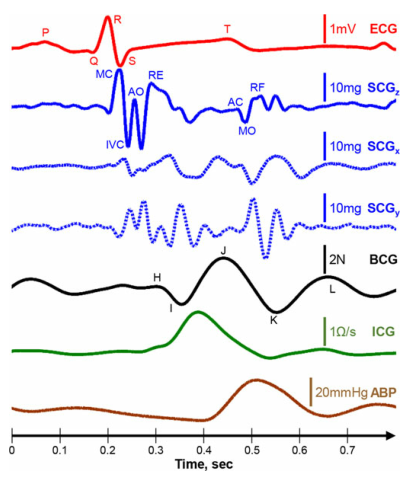
\includegraphics[width=0.4\linewidth]{img/sisBalRevFig1.png}
    \caption{Exemplo de sinal para acelerômetro triaxial, balistocardiogram, eletrocardiograma entre outros}
    \label{fig:sigs}
\end{figure}

    O seismeocardiograma utiliza um medidor de vibrações, geralmente colocado na região torácica, para detectar as movimentações da caixa torácica em resposta aos batimentos cardíacos\cite{ballistoAndSeisReview}. Uma vez que a medição é feita diretamente na região torácica, ela é independente do peso do paciente, mas é fortemente afetada pela inércia do sistema de detecção e por qualquer outro movimento realizado pelo paciente. Considerando os grandes avanços em sensores de acelerômetros realizados nos últimos anos 
%Seria bom ter uma referência e uns dados tipo precisão e massa atual
e dos microcontroladores somos capazes de criar sistemas de medição com grande precisão e pequena inercia que conseguem continuamente ler, armazenar, transmitir e analisar o sinal de aceleração da caixa torácica\cite{06347128}. Como consequência as pesquisas nesse método cresceram, focando inicialmente na detecção de batimento cardíaco contínuo e na padronização dos métodos de medição\cite{06567772}.

     Grande parte das pesquisas atuais tem o foco nas vibrações com direção dorso-ventral, uma vez que essa geralmente trás mais informações relevantes, mas, com o aumento do uso de acelerômetros de três eixos, o estudo paralelo de todos os eixos é possível \cite{3dPrecordialAccSignal}, uma imagem padrão desse sinal pode ser visto na figura: %FIGURA DOS SINAIS PADRÕES DA ballistoAndSeisReview
Um dos grandes problemas desse método, é que, diferente do ECG, seu sinal sofre grandes variações, mesmo quando medidos de um mesmo paciente\cite{3dPrecordialAccSignal}\cite{heartbeatSegInSeismocardiograms}\cite{06945019}, tornando detecções simples, como batimento cardíaco, difíceis e não confiáveis. Um exemplo do sinal de 5 batimentos de dois pacientes, um saudável e outro com isquemia podem ser vistos na figura \ref{fig:5bat}. %Talvez falar um pouco de alguns resultados e do uso de 3d e giroscópio

\begin{figure}[H]
    \center
    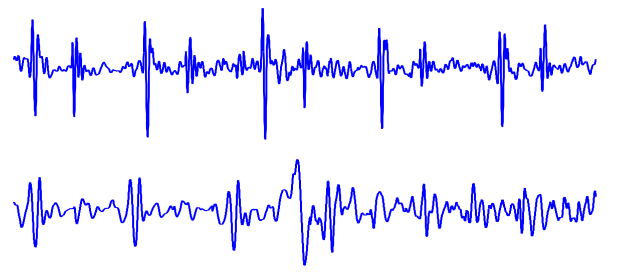
\includegraphics[width=0.4\linewidth]{img/06945019_1.png}
    \caption{sinal do sismeocardiograma de 2 pacientes, durante 5 batimentos cardíacos, o gráfico superior é de um paciente saudável, e o inferior é de um paciente diagnosticado com isquemia}
    \label{fig:5bat}
\end{figure}


    Embora essa dificuldade o sismeocardiograma se apresenta como uma possível alternativa de baixo custo para a análise e monitoramento contínuo e não invasivo da qualidade do ciclo cardíaco do paciente\cite{06611240}, dado que se encontrem caminhos robustos para se interpretarem seus dados sem a necessidade de supervisão humana ou grande quantidade de recursos computacionais

    Um ponto importante a se observar sobre esse três últimos métodos é que todos eles observam o resultado dos movimentos do coração, na sua forma física, tornando possível uma análise do real funcionamento cardíaco, independente do sistema nervoso. Isso poderia levar a possíveis sistemas de diagnósticos poderosos e portáteis, mas somente se algum método de análise for desenvolvido que seja capaz de obter dados significantes e de maneira confiável. 

   \chapter{Objetivo}

    O objetivo desse trabalho é pesquisar técnicas de sensoriamento cardíaco utilizando uma combinação de dados de diferentes sensores para obter informações sobre o ciclo cardíaco de maneira contínua e confiável, tentando inicialmente replicar a confiabilidade do ECG e depois expandir, tentando obter dados mais relevantes sobre o estado do ciclo cardíaco.

    Como discutido na sessão anterior o sismeocardiograma está sendo fortemente estudado, devido à melhoria das tecnologias de acelerômetros e microcontroladores, mas geralmente os dados desse sensor são estudados independente do seu significado físico, sendo observados somente como um sinal elétrico. 
    
    Grande parte das pesquisas leva em consideração somente os dados de um dos eixos de um acelerômetro triaxial, considerando que esse representa a direção dorso-ventral, que deveria onde os movimentos mais relevantes se encontram, mas esse uso simplificado falha em desconsiderar as possíveis variações na direção do acelerômetro. 
    
   Essas variações podem ser resultantes da posição inicial do sensor, que devido a superfície não uniforme da região torácica poderia não estar na direção correta, ou causadas pela variação da direção decorrente do movimento, que, por ser de natureza vibratória, tende a causar alterações na direção do acelerômetro, torando necessário uma correção dessa. %Talvez citar o trabalho de respiração aqui e preciso confirmar esse rolê da vibração

    Mesmo considerando que a posição inicial seja definida com cuidado e que as mudanças de direção não sejam suficientes para gerar uma variação nos dados, a utilização de somente um dos eixos de movimento, ou a utilização dos três independentemente, como é feita em alguns trabalhos, falha em observar o dado pelo que ele é originalmente, e portanto tende a perder informações significativas que podem aparecer ao se levar em consideração que esse dado vem de uma movimentação física de uma sensor com massa e dimensões conhecidas. 

    Portanto proponho utilizar um sensor completo de posicionamento para realizar um seismeocardiograma, analisando a variação de posição do sensor colocado sobre a região torácica ao longo do tempo. Esse sensor seria composto de um acelerômetro, um giroscópio e um magnetômetro, todos triaxiais, e estaria ligado a um microcontrolador, que seria responsável por continuamente ler e armazenar esses dados. 

    Os dados desse sensor serão combinados com o objetivo de gerar uma visão mais completa do movimento cardíaco, tentando reduzir as incertezas e variações apresentadas pelo seismeocardiograma padrão. Essa combinação será feita por algoritmos de filtragem adaptativa como filtros de Kalman e outros, que levam em consideração as origens físicas de cada sensor para obter a posição, mas também por análises matemática, que comparam os dados com um objetivo, por exemplo batimentos cardíacos, e realizam análises iterativa para se localizarem funções que combinam os dados para atingir o objetivo.

    Serão estudados diversas posições para esse sistema, tentando obter informações sobre o movimento cardíaco, colocando sobre a região torácica, informações sobre pressão arterial, colocando sobre artérias próximas a superfície, e algumas outras com o objetivo de obter o maior número de informações complementares sobre o ciclo cardíaco.

   \chapter{Metodologia}

    Considerando o objetivo de combinar os dados do acelerômetro, giroscópio e magnetômetro para obter um dado mais preciso da movimentação causada pelo ciclo cardíaco, o primeiro passo será realizar essa combinação em um ambiente de testes a fim de avaliar os sensores e os algoritmos a serem utilizados e definir se esse método é praticável.

    Antes de considerar as possibilidades de sensoriamento é importante considerar os algoritmos e os dados que esses necessitam. As técnicas que geralmente realizam esse processo utilizam de algoritmos iterativos, que combinam dados de acelerômetros, giroscópios e magnetômetros para atualizar uma estimativa da orientação, considerando um corpo rígido. Esse algoritmo iterativo é geralmente um filtro de Kalman estendido (EKF) baseado em "quaternions" %Colocar alguns artigos
 , mas existem outras alternativas baseadas em diferentes estimadores que também são estudados para esse efeito %Colocar mais artigos
, a fim de conseguir estudar uma variedade de técnicas para conseguir a melhor precisão no caso estudado é necessário um sensor, ou um conjunto de sensores, capaz de realizar a medição de acelerômetro, giroscópio e magnetômetro, com frequência constante e com baixo efeito inercial, dado que as vibrações do sistema cardíaco são pequenas.%Adicionar uma ordem de grandeza
    
    Considerando essas restrições a escolha inicial do sensor será o MPU-9250 da InvenSense (https://www.invensense.com/products/motion-tracking/9-axis/mpu-9250/), esse contêm um acelerômetro, um giroscópio e um magnetômetro, todos de três eixos, com precisão de $16384 LSB/g$, $131 LSB/(º/s)$ e $1,67 LSB/uT$ e ruído de $400 ug/sqrt{Hz}$ e $0.033 º/s-rms$\cite{MPU9250}, e custo de aproximadamente R\$18. Esse sensor foi escolhido baseado na sua grande disponibilidade, na suas características de ruído e precisão, que estão na mesma linha dos acelerômetros utilizados em grande parte dos trabalhos da área, e na sua capacidade de realizar leituras para memória interna, permitindo assim leituras com frequência bem definida. %Talvez citar alguns aqui

    Para estudar o sensor será utilizado um Arduino que será responsável por passar os dados para um computador, que armazenará esses dados. A análise desses dados será feita depois da obtenção, de maneira offline, para que os algoritmos possam ser estudados e corrigidos independentemente do experimento. Os algoritmos estudados serão inicialmente focados no uso do filtro de Kalman estendido, mas, caso necessário, serão expandidos para outras técnicas, a fim de localizar o melhor método de combinação dos sensores, levando em consideração as dimensões reduzidas desses, e a provável existência de movimentos de maior magnitude, como o paciente andando, que vão influenciar fortemente nos resultados.

    Nessa etapa serão realizados experimentos considerando movimentos da mesma ordem de grandeza dos movimentos cardíacos, de forma a se obter dados numéricos da precisão desses métodos quanto a detecção ao longo do tempo. O objetivo final dessa etapa é determinar se o sensor escolhido é capaz de realizar as medições necessárias e determinar qual é a precisão que os algoritmos conseguem atingir, tanto para curtas durações, período de até dois batimentos cardíacos, como para longas durações.  

    Uma vez determinado o sensor e o algoritmo de combinação dos dados, a etapa de análise dos resultados pode ser iniciada, nesse momento o sensor de 9 eixos será colocado na região cardíaca, na posição central%USAR NOMES MELHOR PARA ESSA POSIÇÃO!!!!!!!!
, em conjunto com sensores de referencia, ECG ou fonocardiograma, e os dados de todos eles serão obtidos de forma sincronizada. Considerando que nesse momento cada amostra será formada por aproximadamente por 22 bytes de dados será necessário utilizar um microcontrolador mais capaz.

    Considerando o desejo de que esse sensor seja capaz de funcionar continuamente, o microcontrolador KL25Z-AGMP01 da NXP (http://www.nxp.com/products/sensors/gyroscopes/10-axis-sensor-data-logger-reference-design:RD-KL25-AGMP01) é um bom candidato, uma vez que ele foi criado com o objetivo de ser um coletor de dados, ele já contém bateria recarregável e entrada para microSD, permitindo a aquisição de dados por longos períodos. Além dessas qualidades ele também contém um sensor de 9 eixos embutido, que pode ser utilizado para remoção de movimentos do paciente, considerando que ele esteja na região torácica, mas distante do coração.

    Com esse novo conjunto de dados podemos realizar uma análise sobre os dados do sensor de 9 eixos, comparando ele com os sensores de referência, de forma a definir as informações obtidas por esses. Inicialmente será observado se a análise do sensor de 9 eixos é capaz de obter o batimento cardíaco com precisão e robustez suficiente, depois será estudado se ele é capaz de diferenciar as etapas e eventos do ciclo cardíaco, como o abrir e fechar das válvulas, ou os momentos de sistole e diástole do ventrículo e átrio. Sobre esses resultados serão estudados que outras informações podem ser obtidos, como estimação da variação de pressão entre cada ciclo cardíaco, do volume de sangue ejetado, entre outros.

    Além disso também será estudado a capacidade de se obter essas informações de modo contínuo, ou seja, com o paciente em movimento normal na sua rotina. Para essa etapa será utilizado o sensor de 9 eixos fora da região cardíaca para se estimar o movimento geral do corpo e remover esse dos dados.

    Por final espera-se obter uma definição da factibilidade e utilidade desse método de sensoriamento da condição cardíaca por meio de localização da posição torácica, além de obter um estudo detalhado sobre o uso do sensor de 9 eixos para a localização em pequena escala. 

   %\input{sweep.tex}
    %\input{tr.tex}
    %\input{solucaoInversa.tex}
    %\input{sim.tex}
    %\input{simIH.tex}
    \bibliography{b}{}
    \bibliographystyle{plain}
%Projeto de pesquisa de Mestrado realizado pelo aluno Bernardo Mascarenhas Camargos e Silva com orientação do professor Sérgio Shiguemi Furuie, realizado no dia \today
%
%\vspace{21cm}
%\noindent\begin{tabular}{ll}
%\\[6ex]
%\makebox[3in]{\hrulefill} &\hspace{1.5cm} \makebox[9cm][l]{\hrulefill}\\
%Sérgio Shiguemi Furuie (Orientador)  & \hspace{1.5cm} Bernardo Mascarenhas Camargos e Silva (Aluno)
%\end{tabular}

\end{document}
